% 2011 大纲卷(文) 第22题 图: 椭圆、过焦点的直线l与线段OA,OB
\usetikzlibrary{arrows.meta,calc}
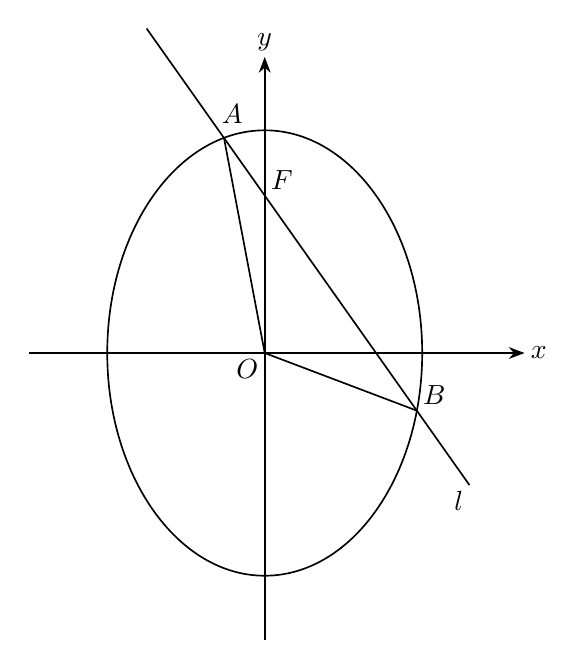
\begin{tikzpicture}[x=1cm,y=1cm,line width=.6pt,font=\normalsize,>=Stealth]
%==DATA-START== do not reorder
\def\scale{2.0}
\def\ellRx{2.0}
\def\ellRy{2.8284271247461903}
\coordinate (O) at (0.0,0.0);
\coordinate (F) at (0.0,2.0);
\coordinate (A) at (-0.5176380902050414,2.732050807568877);
\coordinate (B) at (1.9318516525781364,-0.7320508075688772);
\coordinate (Lone) at (-1.5,4.121320343559643);
\coordinate (Ltwo) at (2.6,-1.6769552621700474);
\coordinate (Xone) at (-3.0,0.0);
\coordinate (Xtwo) at (3.3,0.0);
\coordinate (Yone) at (0.0,-3.64);
\coordinate (Ytwo) at (0.0,3.76);
%==DATA-END==
\draw[->] (Xone)--(Xtwo) node[right=2pt,inner sep=0pt] {$x$};
\draw[->] (Yone)--(Ytwo) node[above=2pt,inner sep=0pt] {$y$};
\draw (O) ellipse ({\ellRx} and {\ellRy});
\draw (Lone)--(Ltwo);
\draw (O)--(A);
\draw (O)--(B);
\node[below left,inner sep=0pt,xshift=-2pt,yshift=-2pt] at (O) {$O$};
\node[anchor=south,inner sep=0pt,xshift=3pt,yshift=5pt] at (A) {$A$};
\node[above right,inner sep=0pt,xshift=2pt,yshift=2pt] at (F) {$F$};
\node[above right,inner sep=0pt,xshift=2pt,yshift=2pt] at (B) {$B$};
\node[below left,inner sep=0pt,xshift=-2pt,yshift=-2pt] at (Ltwo) {$l$};
\end{tikzpicture}
